\documentclass[12pt,a4paper,english,onecolumn]{IEEEtran}

\usepackage{datetime}
\usepackage{caption}
\usepackage{graphics}
\usepackage{color}
\usepackage{graphicx}
\usepackage{listings}
\usepackage{minted}
\usepackage{hyperref}
\usepackage[utf8]{inputenc}
\usepackage{wrapfig}
\usepackage[paper=a4paper, top=2cm, bottom=3cm, left=2.5cm, right=2.5cm]{geometry}
\usepackage[
    backend=bibtex,
    style=numeric,
    bibencoding=ascii,
    sorting=ynt
]{biblatex}
\addbibresource{bibliography}
\usepackage[scale=0.95]{droidsansmono}

\definecolor{ao}{rgb}{0.0, 0.5, 0.0}

\renewcommand*\contentsname{Table of Content}
\renewcommand*\listfigurename{List of Images}
\renewcommand\listingscaption{Example}
\renewcommand{\listtablename}{List of Tables}
\captionsetup[table]{name=Table}
\renewcommand*\figurename{Image}
\usemintedstyle{bw}
\hyphenpenalty=100000
\nocite{*}
\usepackage[T1]{fontenc}

\begin{document}
\lstset{
language=C,                             % Code langugage
basicstyle=\ttfamily,                   % Code font, Examples: \footnotesize, \ttfamily
keywordstyle=\color{blue},        % Keywords font ('*' = uppercase)
commentstyle=\color{ao},              % Comments font
stepnumber=1,                           % Step between two line-numbers
numbersep=2pt,                          % How far are line-numbers from code
frame=none,                             % A frame around the code
tabsize=1,                              % Default tab size
captionpos=b,                           % Caption-position = bottom
breaklines=false,                        % Automatic line breaking?
breakatwhitespace=false,                % Automatic breaks only at whitespace?
showspaces=false,                       % Dont make spaces visible
showtabs=false,                         % Dont make tabls visible
}


\title{\Large\textbf{{CVE-2014-0160}} \\
\large{The Heartbleed Bug} \\
\vspace{10px}
\small{https://nvd.nist.gov/vuln/detail/cve-2014-0160}
}

\author{Dragoș IOANA$^{1}$, Adina VAMAN$^{2}$\\
$^{1, 2}$\emph{Politehnica University of Bucharest, Computer Science Department, Romania}\\
Email: $^{1}$dragos.ioana@stud.acs.upb.ro, $^{2}$adina.vaman@stud.acs.upb.ro}

\maketitle

\begin{abstract}

The Heartbleed vulnerability is one of the most significant since the Internet started to be used commercially. It compromised a considerable amount of private data, from certificates to passwords and other authentication tokens. This paper aims to go over the background and the initial discovery of the vulnerability, followed by a description of the faulty implementation and means of exploitation. In Chapter IV, we summarize the effects that Heartbleed had over the Internet as a whole. Finally, we end with a Proof-of-Concept implementation that puts theory into practice.

\end{abstract}

\section{Introduction}

In March 2014, researchers found a catastrophic vulnerability in \textbf{OpenSSL}, a cryptographic library that has been widely used to implement the \textbf{Transport Layer Security} (TLS) protocol. It is described by some as being the worst vulnerability since commercial traffic began to flow on the Internet [3]. OpenSSL was integrated in popular server products such as Apache and Nginx, therefore allowing attackers to remotely read protected memory from an estimated 24-55\% of popular HTTPS websites [4]. The bug is simple to understand and exploit, thus exacerbating its severity. \par
The bug resulted from \textbf{improper input validation} in the implementation of the TLS heartbeat extension, proposed as a standard in February 2022 by \textbf{RFC 6520} [2]. The heartbeat extension aimed to allow the usage of keep-alive functionality in the \textbf{Datagram Transport Layer Security} (DTLS), which was meant to secure unreliable datagram traffic. This extension was necessary in order to provide functionality similar to TLS run over TCP traffic, that already provided session management.\par
On the surface, \textbf{Heartbleed} is essentially a \textbf{buffer overread vulnerability}, where inadequate bounds checking is carried out at runtime. Another way of looking at the problem is that the programmers placed trust in user input, meaning that they assumed that the end user would not specify a payload length larger than the payload itself. Placing trust in user input is not a good philosophy, making \textbf{sanitization and bounds checking} extremely important. \par
The Heartbleed vulnerability was originally found in March 2014 by Neel Mehta of Google’s security team, who then reported it privately to the OpenSSL team on 1st of April 2014. Around the same time, the Finnish cybersecurity company Codenomicon also discovered the bug independently, reporting 3 April 2014 as their date of discovery. In turn, they also were the ones to name the bug, to create the bleeding heart logo and to explain the bug to the public through a website [5]. The public disclosure of Heartbleed started on April 7, 2014, when the OpenSSL core team decided to release a patched version 1.0.1g, followed by a public security advisory [4]. \par



\vspace{10px}

\section{Related Work}

After the public disclosure of Heartbleed, researchers have been quick to analyze the causes, the mitigation and the effects of this very high-profile vulnerability. One of the most notable papers that provide a comprehensive analysis of Heartbleed is \textbf{The Matter of Heartbleed} [2], authored by Zakir Durumeric, Frank Li et. al. It was published in November 5, 2014, a few months after the initial discovery was made. It provides extensive information about the reasoning behind the TLS Heartbeat extension and the implementation at fault for the vulnerability. In Section 2.4, it also describes the events that took place around the time of the discovery and how the information was disclosed between parties. From Section 3 onwards, authors describe how they scanned all of the Alexa Top 1 Million websites in different points in time in order to check whether they are still vulnerable to Heartbleed. They monitor how websites began to patch their servers, also going over the general impact that the bug has had over Internet as a whole, over the certificate ecosystem or over mail servers.


 \section{Attack description}

The Heartbleed vulnerability was found in the TLS Heartbeat extension, proposed as a standard in February 2022 by RFC 6520 [2]. It was meant to allow either endpoint of a TLS connection to detect whether its peer is still present, since the Datagram TLS protocol run over UDP did not provide session management. Standard implementations of TLS do not need this extension, since they can rely on TCP for the session management functionality. Version 1.0.1 of OpenSSL, released on March 14, 2012, added support for the Heartbeat functionality and enabled it by default, thus inadvertently making computers running it vulnerable to the bug. \par
During the initial TLS handshake, the peers negotiate whether they support the Heartbeat extension. After the initial negotiation and handshake is finished, either peer can send a HeartbeatRequest message to verify whether the other is still connected. HeartbeatRequest messages consist of a two-byte payload length field, the payload itself, and at least 16 bytes of random padding. The receiving peer is expected to respond with a similar HeartbeatResponse, which contains the same payload received and a newly-generated random padding. \par
\vspace{5px}
\begin{wrapfigure}{l}{0.52\textwidth}
  \begin{center}
    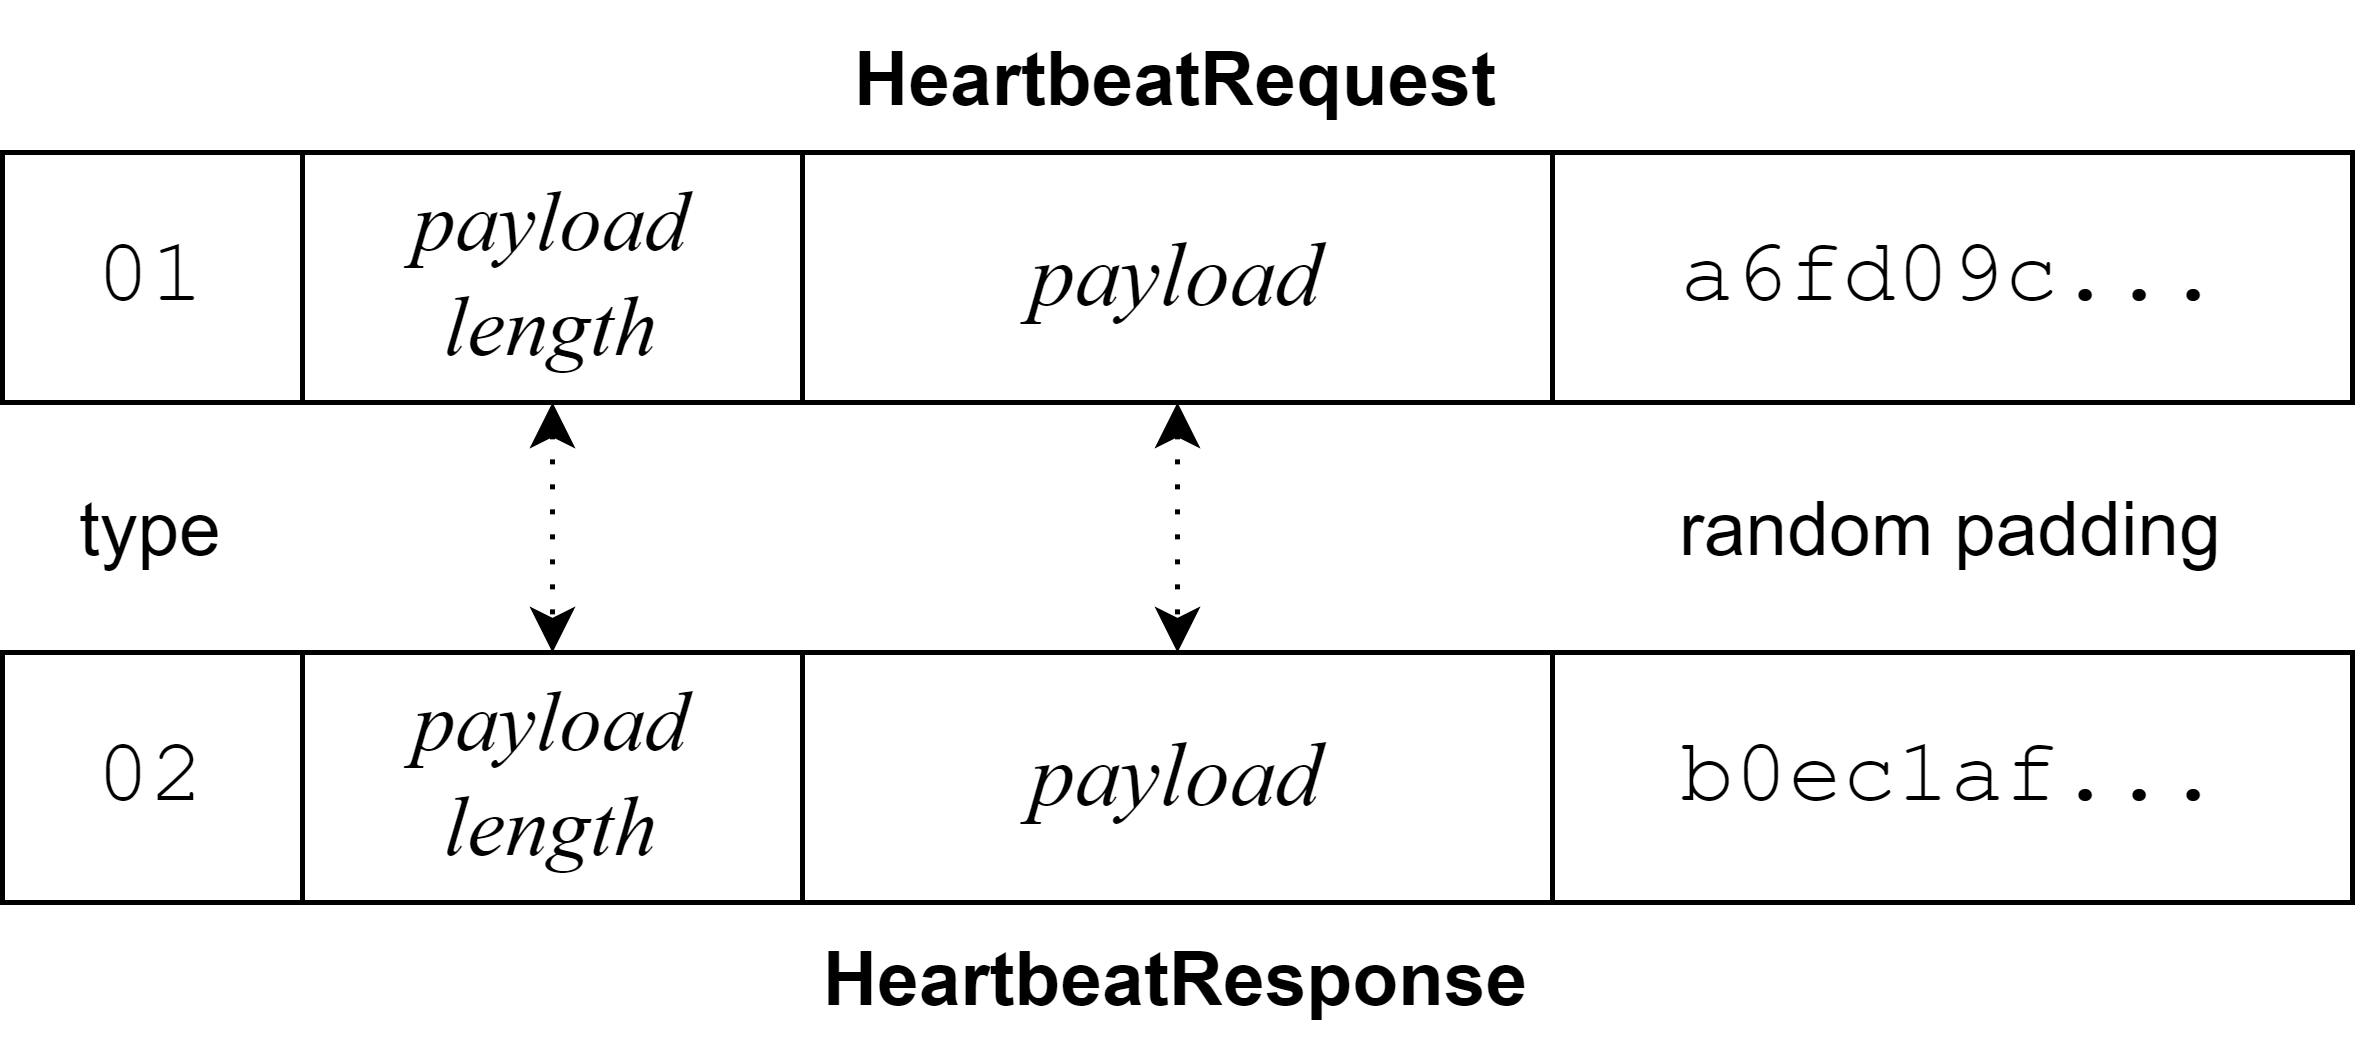
\includegraphics[scale=0.1]{images/heartbeat-packet.png}
  \end{center}
  \caption{Heartbeat message structure}
\end{wrapfigure}
However, the faulty implementation did not check whether the payload length field actually corresponded with the length of the data inside the payload field. Upon receiving a HeartbeatRequest message, the peer responds with a payload length number of bytes, regardless of the fact that the length indicated in the request is bigger than the actual payload. Therefore, the other endpoint can access private data stored directly after the payload by specifying a payload length larger than the payload itself. Since the size of the payload length field is two bytes, an attacker can obtain up to $2^{16}$ bytes (64 KB) of memory in a single message. Thus, the vulnerability allows the attacker to consistently access private memory, that can include private keys or other data that has been transferred over a secure channel. \par
The patched version of OpenSSL adds a bounds check that verifies whether the payload length field is larger than the field of the payload. If there is any inconsistency, the message is then discarded silently. \par

\begin{figure}[!htb]
\noindent\begin{minipage}[b]{0.4\textwidth}
\begin{lstlisting}[]
    hbtype = *p++;
    n2s(p, payload);
    pl = p;
    memcpy(bp, pl, payload);
\end{lstlisting}
\caption*{OpenSSL 1.0.1a-1.0.1f versions}
\end{minipage}%
\hfill
\noindent\begin{minipage}[b]{0.45\textwidth}
\begin{lstlisting}[]
    hbtype = *p++;
    n2s(p, payload);
    if (1 + 2 + payload + 16>
        s->s3->rrec.length)
    /* silently discard per
    RFC 6520 sec. 4 */
      return 0; 
    pl = p;
    memcpy(bp, pl, payload);
\end{lstlisting}
\caption*{OpenSSL 1.0.1g bounds check}
\end{minipage}%
\end{figure} 

\vspace{30px}
\section{Effects}

The Heartbleed vulnerability was catastrophic due to its simplicity and the ubiquity of OpenSSL across web servers. It has been estimated [4]  that up to 55\% of HTTPS servers in the Alexa Top 1 Million were initially vulnerable, including 44 of the Alexa Top 100. Even prior to the public disclosure of the bug, some companies found out about the matter in advance. Neel Mehta, a Google cyber security employee, was the first to find the Heartbleed vulnerability on March 21, 2014, more than two years after the initial release of the TLS Heartbeat extension. However, this discovery was originally kept private by Google as part of responsible disclosure efforts; they followed to patch OpenSSL on their servers the same day as the discovery was made. Then, news of the bug spread privately among inner tech circles. On March 31, CloudFlare was privately notified, and the company also patched their servers the same day. Finally, the OpenSSL core team was privately notified on April 1st. The following day, the Finnish company Codenomicon independently discovered the bug and reported it to the National Cyber Security Centre of Finland. They also gave the vulnerability its name and purchased the heartbleed.com domain in order to spread awareness. After having been notified twice by two separate entities about the vulnerability, the OpenSSL core team decided to release a patched version and to commence the public disclosure of Heartbleed. \par
	Heartbleed could potentially affect any service that used OpenSSL in order to facilitate TLS connection. TLS implementations other than OpenSSL’s, such as GnuTLS, Mozilla’s Network Security Services and the Windows platform implementation of TLS were not affected, as the issue existed in the OpenSSL implementation of TLS rather than in the protocol itself. \par
The data obtained by a Heartbleed attack can reveal any form post data in the users' requests, private keys of compromised parties, or even session cookies and passwords. This can allow an attacker to then impersonate a user of the service or decrypt future or past stored traffic with the obtained cryptographic keys. Even if the victim itself patched the vulnerability, an attacker who obtained authentication material could still impersonate the material’s owner as long as the server is still accepting the material. Thus, as long as the password is not changed or the private key is revoked, the online account is still compromised, making Heartbleed a critical threat to confidentiality. Moreover, domain certificates could also be compromised in the same way by leaking their private keys. Therefore, any server susceptible to Heartbleed should have their certificates revoked and reissued. \par

\section{Attack mitigation}

After the public reveal of the bug, OpenSSL released the patched version 1.0.1g on April 4, 2014, almost two years after the release of version 1.0.1 which introduced the Heartbeat functionality along with the vulnerability. Therefore, remediation of the bug is basically resolved by updating OpenSSL to a patched version. Since OpenSSL can be used in means such as a standalone program, a dynamically-linked shared object or a statically-linked library, all of them must be taken into account for mitigating the vulnerability. All programs and libraries which use the statically-linked version must be stopped, relinked and restarted, and packages which have OpenSSL as a dependency must be updated. Moreover, after patching the programs, they must be restarted in order to remove the in-memory copy of the old, vulnerable copy of the OpenSSL code. \par
	Simply patching the vulnerable code is not enough for remediating all the effects of Heartbleed. Since the vulnerability exposes any type of private data, from session cookies to passwords and private keys, server administrators must address each possible breach of confidentiality. Private keys must be treated as compromised and thus key pairs must be regenerated; moreover, certificates that use them must be revoked and reissued. Passwords and other authentication material could have also been compromised and should also be regenerated. These measures should be done proactively, since it is nearly impossible to tell whether certain information was leaked or not. \par
	According to [4], an estimated 24-55\% of HTTPS servers in the Alexa Top 1 Million were initially vulnerable, including 44 of the Alexa Top 100. The same source states that two days after disclosure, 11\% of HTTPS sites in the Alexa Top 1 Million remained vulnerable, as did 6\% of all HTTPS servers in the public IPv4 address space. Within the first 24 hours, all but 5 of the Alexa Top 100 sites were patched and within two days, all of the vulnerable hosts in the top 500 were patched. Two months after the public disclosure, 3\% of HTTPS sites in the Alexa Top 1 Million still remained vulnerable. \par

\section{Proof-of-Concept description and implementation}

In order for the exploit to be demonstrated, the following setup was made: creating an Apache server that has the SSL module enabled and configured with a vulnerable version of OpenSSL, 1.0.1e for this example, and a C script which simulates the TLS handshake between the server and a created socket, enables the Heartbeat extension and sends requests with no payload, but $2^{16} - 1$ payload length with the purpose of the server echoing back sensitive information. \par
The server was created inside a container using Dockerfile as a build context, and uses a Linux Debian:Jessie base image,a version released in early 2015 and compatible with the 1.0.1 versions of OpenSSL. Due to the fact that this bug was initially pointed out in 2014 and resolved the very same year, necessary tools needed to be installed from archived snapshots. A simple login page written in HTML and Javascript, that stores the information given through user interaction inside cookies was used to demonstrate the potency of this attack.
Downloading the source files for each of necessary tools, namely OpenSSL and the httpd server, building them and then using the install scripts generated was to setup the vulnerable server, was another possibility. \par
    The main focus of the PoC is the exploit script, having been implemented with the information found in \textbf{RFC 5246}[1] regarding the TLS v1.2 messages format and \textbf{RFC 6520}[2] regarding the structure of Heartbeat messages. The main steps taken to reproduce an attack were the socket creation, \textbf{Client Hello} packet crafting to create a session that uses the Heartbeat extension, TLS handshake realization by reading the record layer header and comparing the content type identified with the values described in section 7.4 of RFC 5246[1] until a \textbf{Server Hello Done} message is received, marking the end of the handshake and that an encrypted channel has been created. When the previous steps have ended, all that remains is sending the server a spoofed Heartbeat request, whose payload length is the maximum permitted value, $2^{16}$ bytes, with no actual payload included, to which the server will respond with $2^{16}$ bytes from its memory, that might contain session identifiers, cookie values or keys.

\section{results}

Using the aforementioned implementation, the instantiation of a Docker container with the builded image, and entering of a set of fake credentials from the browser into the HTML page served by the Apache, is required for the exploit to work. In doing this, the browser saved information in two cookies: one for the username and one for the password. After this initial step, all that needed to be done is run the exploit, which also contains a hexdump functionality to facilitate printable character reading from the server information dump. When receiving the Heartbeat response, the script looks for a particular sequence of bytes, representing the name of a cookie, and then saves in a text file all the information. \par

Examining the saved file, we notice that non printable byte-chunks predominate but they are intercalated with useful information regarding HTTP request headers, status message and also the cookies' names and associated values.

\vspace{10px}
\section{References}
\nocite{*}
\printbibliography[heading=none]

\end{document}
